\break

\hypertarget{biosketches}{%
\section*{Biosketches}\label{biosketches}}
\addcontentsline{toc}{section}{Biosketches}

\textbf{Ruan van Mazijk} is a Masters student broadly interested in
comparative biology and \ldots{}

\textbf{Michael D. Cramer}

\textbf{G. Anthony Verboom}

\hypertarget{author-contributions}{%
\section*{Author contributions}\label{author-contributions}}
\addcontentsline{toc}{section}{Author contributions}

MDC and GAV conceived the study question, which RVM investigated under
their supervision for his BSc Hons project. The analyses and programming
work were largely devised by RVM, with input from the other authors, and
was carried out by RVM. RVM wrote the first draft of the manuscript and
all authors contributed equally thereafter.

\hypertarget{orcid-numbers}{%
\section*{ORCID numbers}\label{orcid-numbers}}
\addcontentsline{toc}{section}{ORCID numbers}

RVM: 0000-0003-2659-6909

MDC: 0000-0003-0989-3266

GAV: 0000-0002-1363-9781

\hypertarget{figures}{%
\section*{Figures}\label{figures}}
\addcontentsline{toc}{section}{Figures}

\begin{figure}[H]
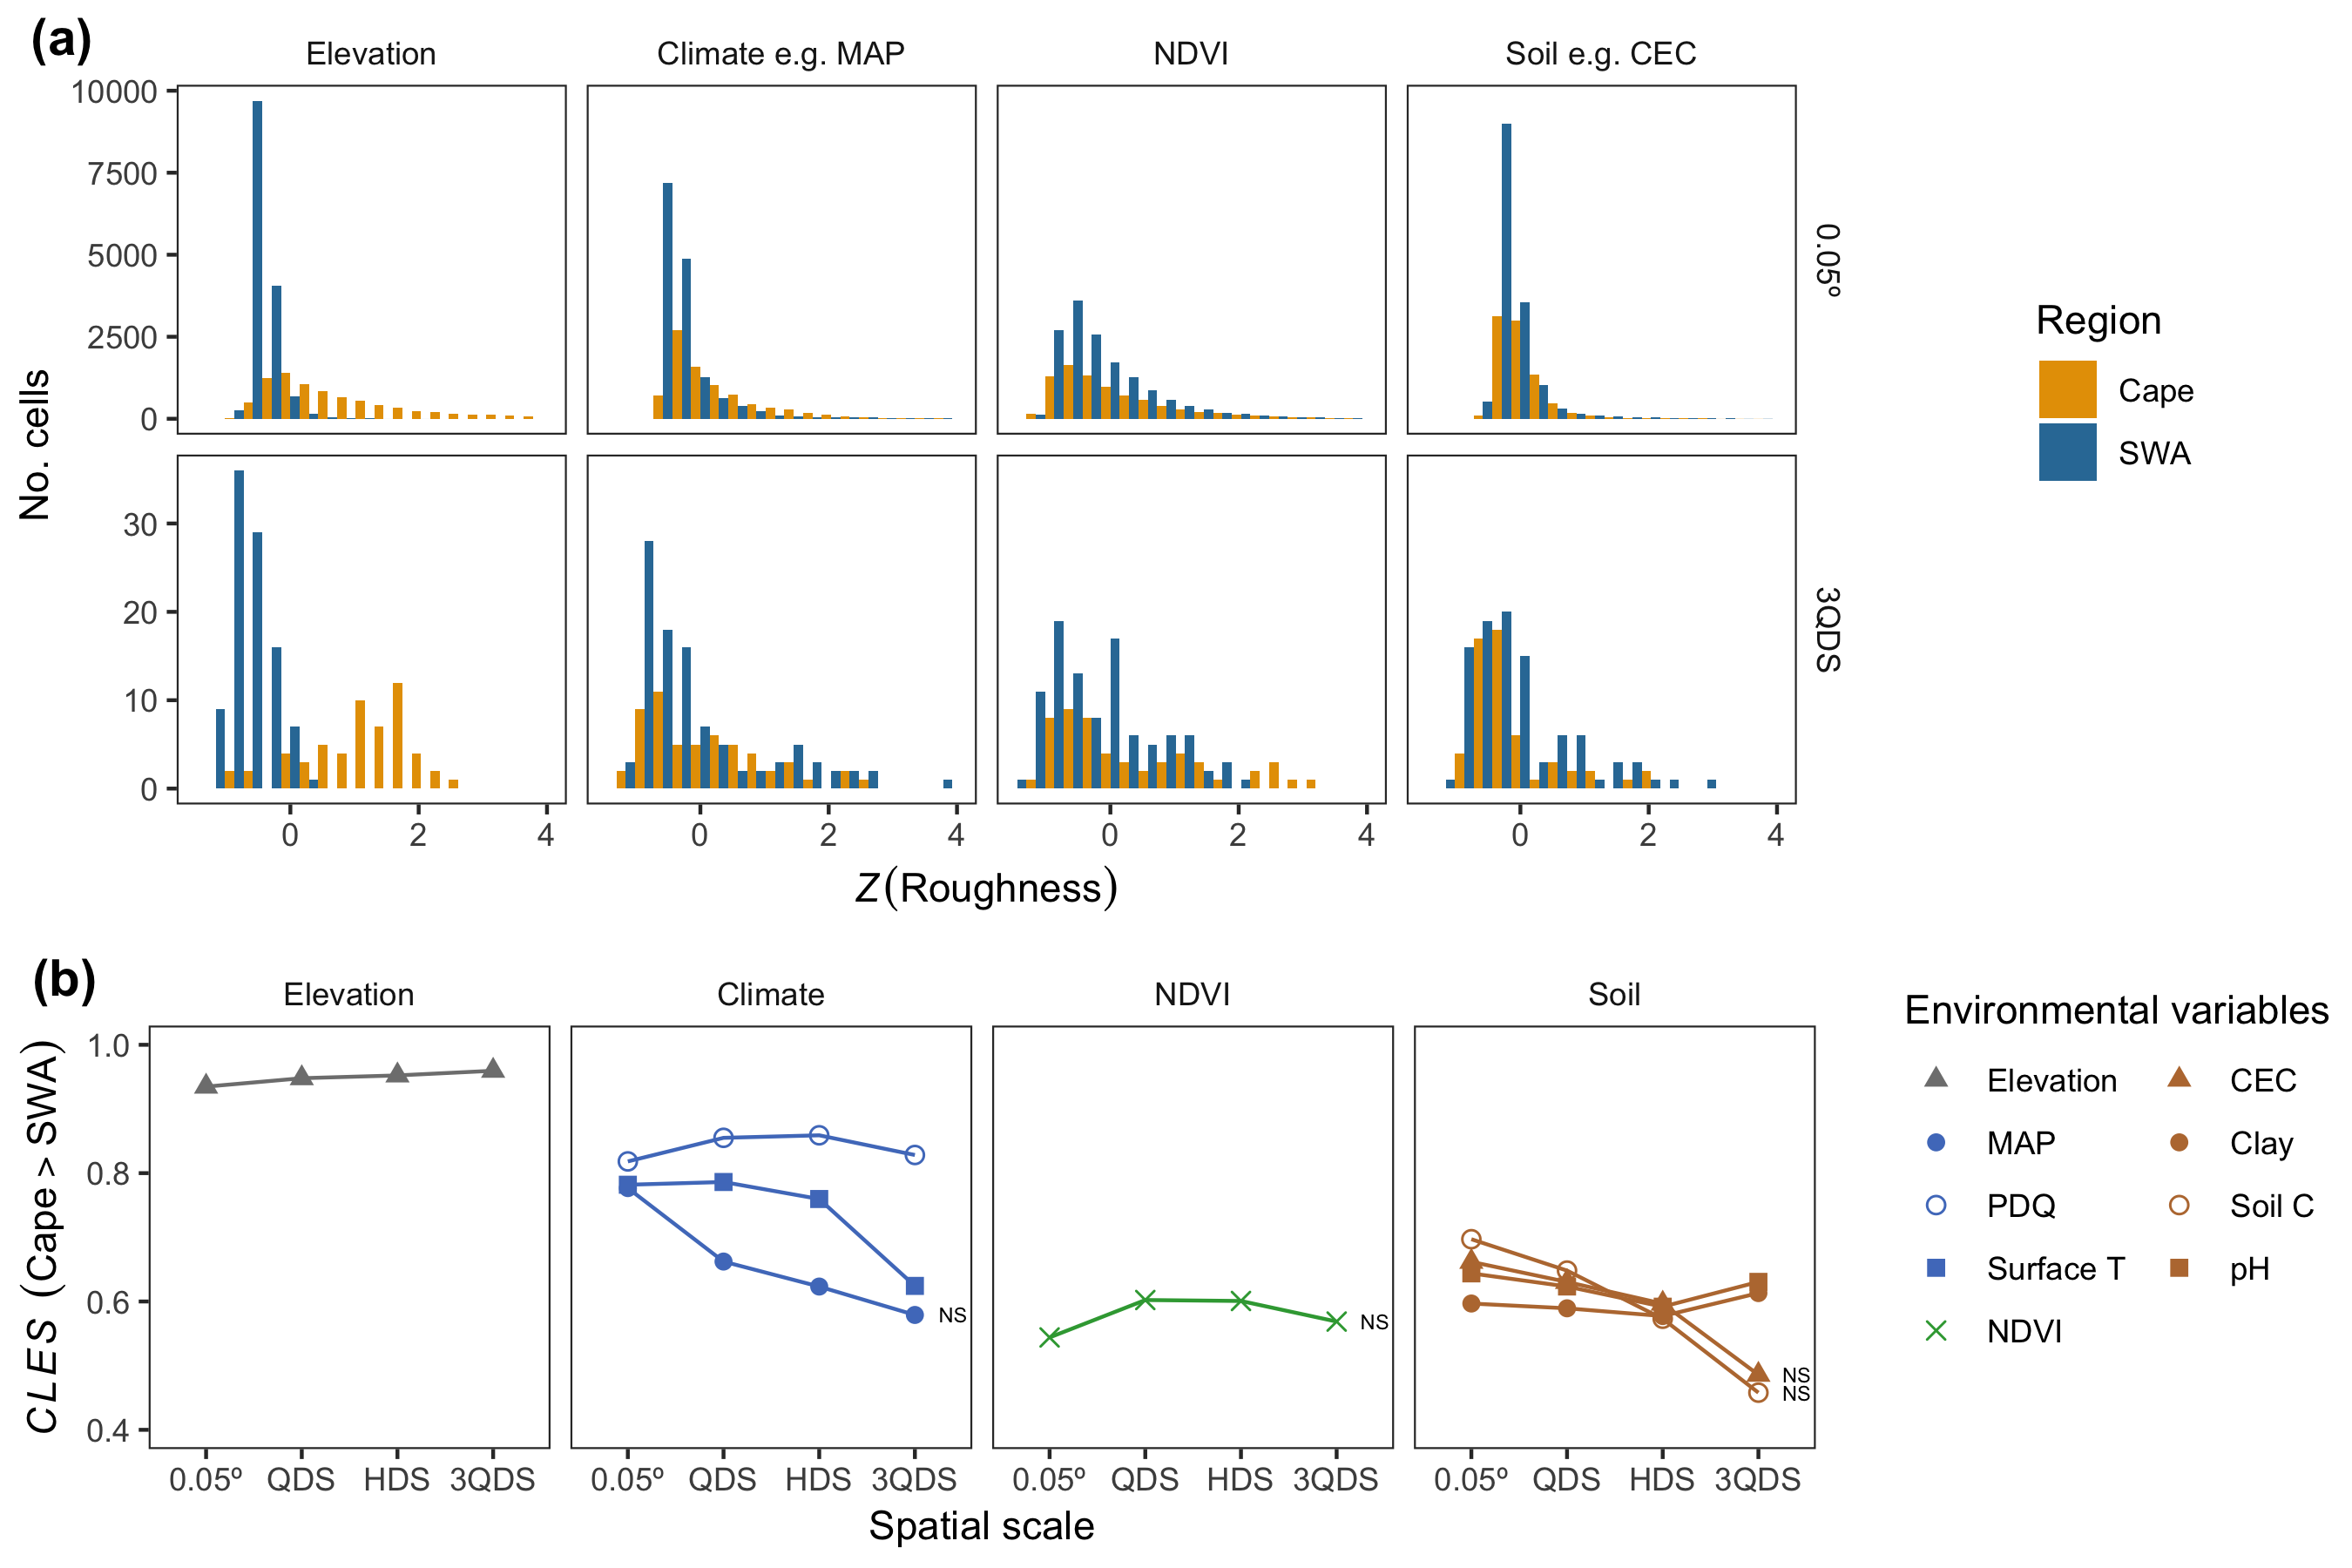
\includegraphics[width=18cm]{/Users/ruanvanmazijk/projects/Cape-vs-SWA/figures/fig-1-roughness} \caption{(ref:roughness)}\label{fig:roughness}
\end{figure}

\begin{figure}[H]
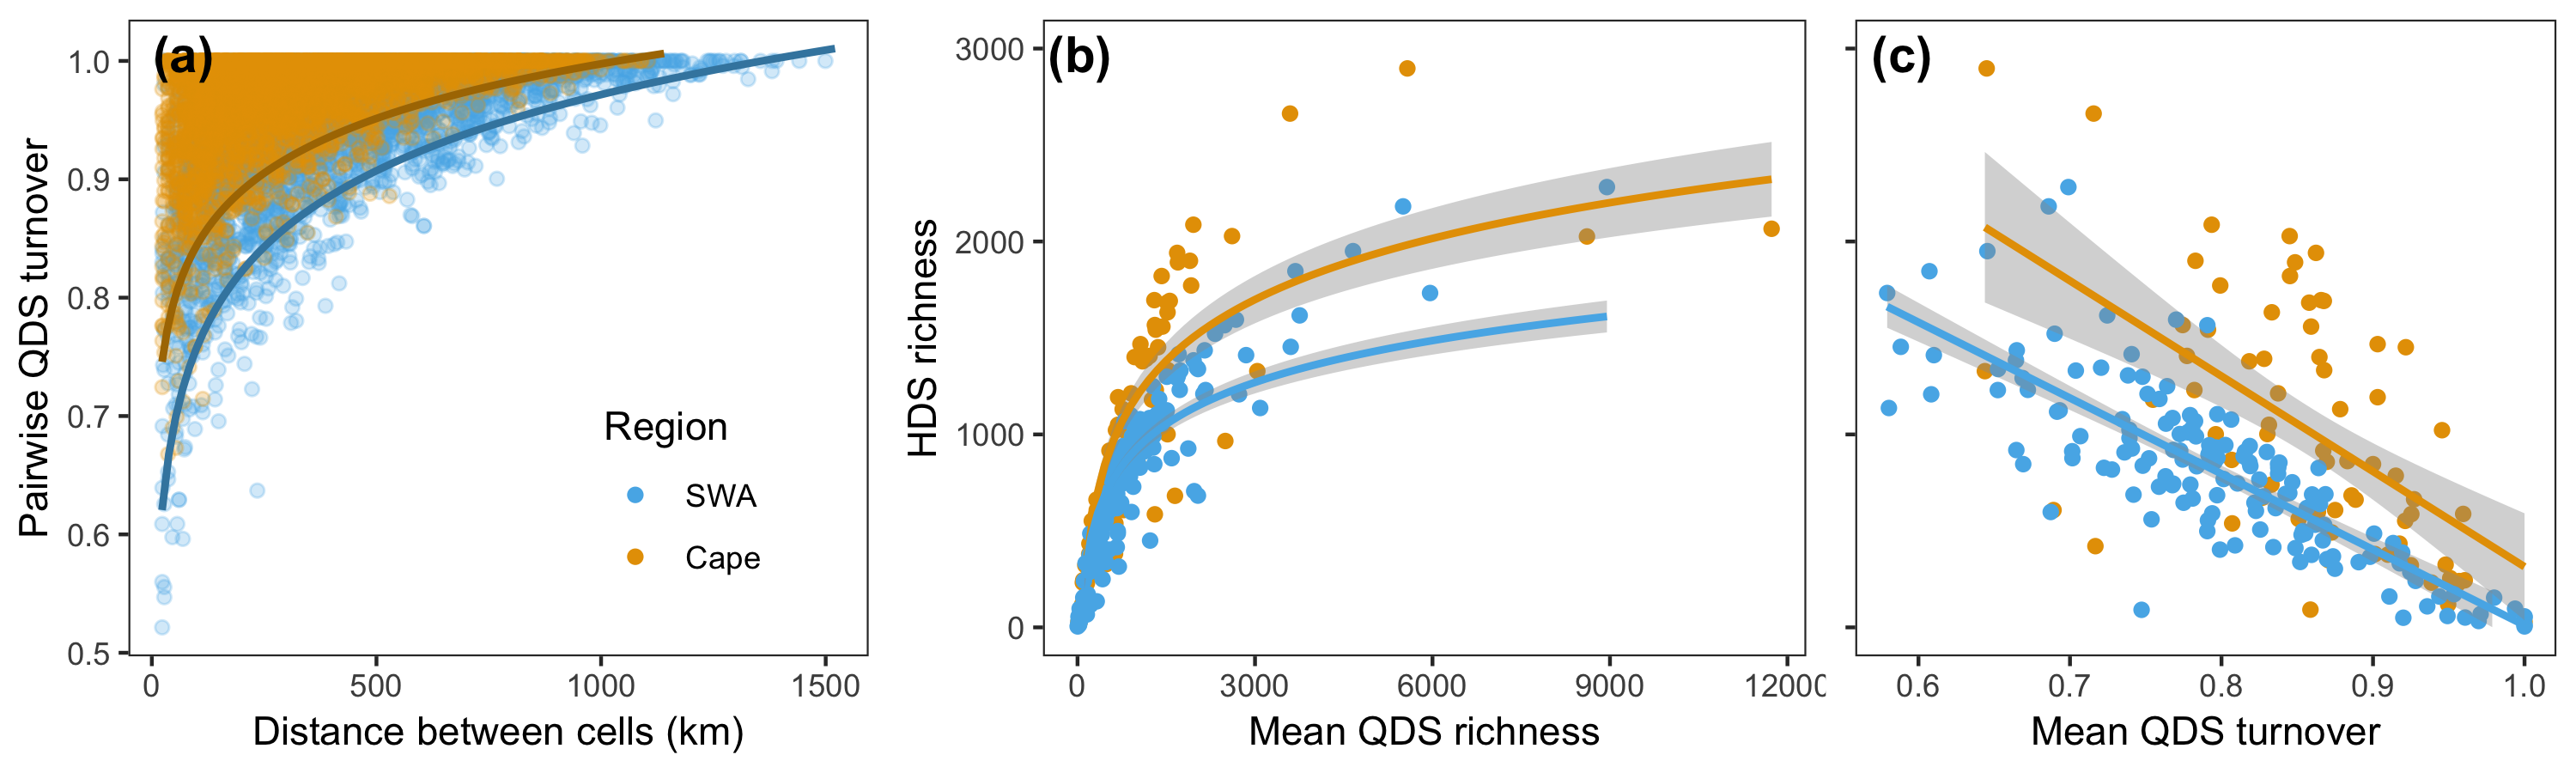
\includegraphics[width=18cm]{/Users/ruanvanmazijk/projects/Cape-vs-SWA/figures/fig-2-richness-vs-turnover} \caption{(ref:richness-vs-turnover)}\label{fig:richness-vs-turnover}
\end{figure}
